\chapter{Previous Works, Discussions, and Findings}

\section{Background Study}

\subsection{CNN}

A \ac{cnn} is a specialized artificial neural network designed primarily for processing structured grid-like data, such as images. Unlike traditional neural networks, CNNs are specifically tailored to capture spatial hierarchies and patterns in data through a series of convolutional layers, pooling layers, and fully connected layers.

\begin{figure}[h]
    \centering
    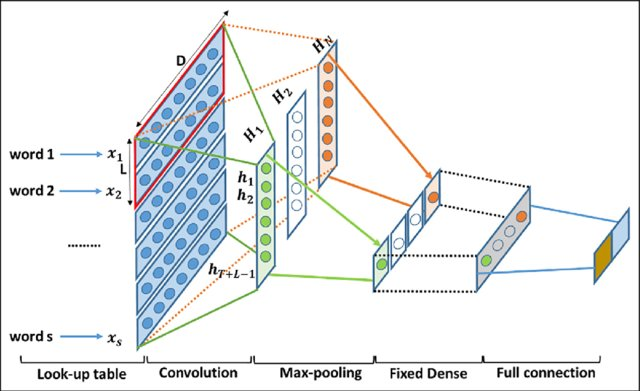
\includegraphics[scale=1.2]{CNN architecture.jpg}
    \caption{CNN architecture}
    \label{fig:cnn artchitecture}
\end{figure}

\begin{description}

    \item[1. Convolutional layer:] The convolutional layer applies convolutional operations to sequential data, such as sentences or documents. The input is typically a matrix where each row represents a word encoded as a vector, often using word embeddings like Word2Vec, \ac{glove}. The convolutional layer uses filters (kernels) of various widths that slide over the input text to capture local patterns and n-grams.

    \item[2. Pooling layer:] Pooling layers, such as max pooling, are often used to downsample the feature maps, reducing their dimensionality while retaining the most critical features. For text, max pooling is commonly used to capture the most important feature (e.g., the highest value) from each feature map, regardless of its position.
   
    \item[3. Fully connected layers:] These layers, typically found at the end of the network, connect every neuron in one layer to every neuron in the next layer. They are responsible for combining the extracted features to make the final classification or prediction.
       
\end{description}

\subsection{CNN-LSTM}

Combining \ac{cnn} with \ac{lstm} networks is a powerful technique for handling data with spatial and temporal dependencies. The CNN-LSTM architecture leverages the strengths of both CNNs and LSTMs to handle complex data with spatial and temporal characteristics. The output of the CNN layer (i.e. the feature maps) is the input for the \ac{rnn} layer of LSTM units/cells that follow. The RNN layer uses the local features extracted by CNN and learns the long-term dependencies of the local features of news articles to classify them as fake or real. The proposed model is depicted in fig \ref{fig:cnn-lstm}. \\

\begin{figure}[h]
    \centering
    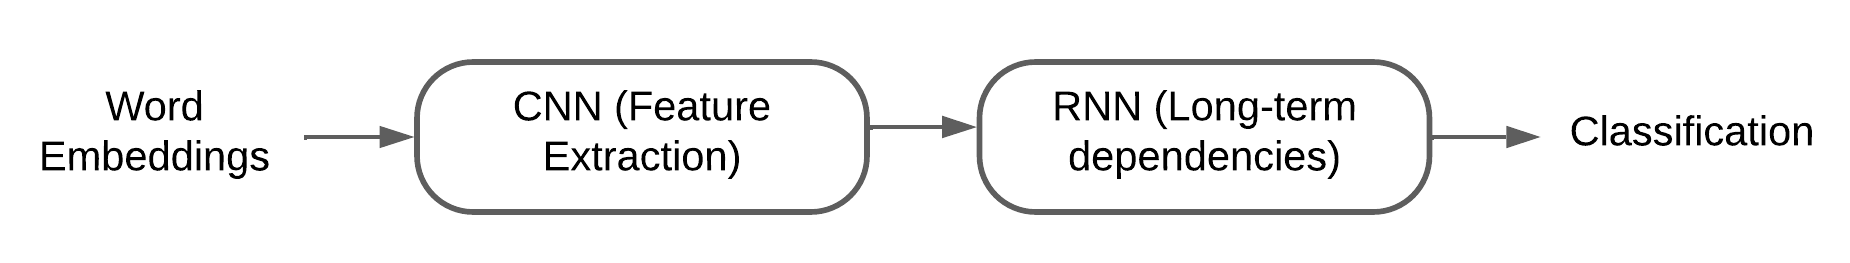
\includegraphics[scale=0.9]{cnn-rnn.png}
    \caption{CNN-LSTM}
    \label{fig:cnn-lstm}
\end{figure}

The LSTM consists of the following control gates :

\begin{description}

    \item[1. Input gate:] The input gate determines which values from the input should be used to modify the memory. It utilizes a sigmoid function to decide which values to let through (ranging from 0 to 1) and a tanh function to assign weights to the values, indicating their level of importance.

    \item[2. Forget gate:] The forget gate determines what information should be discarded from the memory cell. It also employs a sigmoid function, which looks at the previous state and current input, and outputs values between 0 (omit this information) and 1 (keep this information) for each element in the memory cell state.
   
    \item[3. Output gate:] The output gate combines the input and memory of the LSTM block to determine the output. It uses a sigmoid function to decide which values to pass through (ranging from 0 to 1) and a tanh function assigns weights to the values, indicating their level of importance. The weighted values are then multiplied with the output of the sigmoid function to generate the final output.
       
\end{description}

\subsection{CNN-Attention}

Combining \ac{cnn} with attention mechanisms is a powerful approach to enhance the ability of CNNs to focus on the most relevant parts of the input data. Attention mechanisms enable models to focus on the most relevant parts of the input data, dynamically weighing different parts based on their importance.

\begin{description}

    \item[1. Attention layer:] The attention mechanism computes attention scores for the feature maps generated by the CNN. These scores indicate the relevance of each feature in the context of the classification task. The attention mechanism enables the model to focus on the most important parts of the text, enhancing its ability to capture global context and long-range dependencies. The attention scores are used to compute a weighted sum of the feature maps, producing a context vector that represents the most relevant features of the text.
    
\end{description}

\section{Literature Review}

Fake news detection has become an essential area of research due to the rapid spread of misinformation through social media and online news platforms. \ac{cnn}, originally designed for image processing, has shown significant promise in text classification tasks, including fake news detection. This literature review explores key developments, methodologies, and findings in using CNNs for detecting fake news.\\

Yoon Kim's seminal paper applied CNNs to sentence classification tasks. The model used static and dynamic word embeddings, and multiple filter sizes to capture various n-gram features. The study showed that CNNs could capture important local features and patterns in text data, which are crucial for distinguishing between fake and real news \cite{kim2014convolutional}. Wang extended the application of CNNs to fake news detection by training a CNN model on the LIAR dataset. This study highlighted CNN's ability to learn intricate patterns in the text that are indicative of false or fake news, such as sensational language and specific word usage \cite{wang-2017-liar}. \\

The study \cite{zhang2016characterlevel} proposed using CNNs directly on character-level text, bypassing the need for word embeddings. The model showed that character-level representations could be effective for text classification, especially in cases where word-level information might be sparse or noisy. Conneau and colleagues proposed using very deep CNNs with up to 29 convolutional layers. They demonstrated that deeper networks, along with residual connections, could capture more complex features and improve text classification accuracy \cite{conneau2017deep}.\\

Combining CNNs with RNNs leverages the strengths of both architectures: CNNs for local feature extraction and RNNs for capturing sequential dependencies. Lai et al. introduced a Recurrent Convolutional Neural Network (RCNN) for text classification, which improved performance by combining convolutional and recurrent layers  \cite{Lai2015RecurrentCN}.  The research by Nasir et al. shows the use of a hybrid CNN-RNN model on two fake-news datasets (ISO and FA-KES) with better detection results than other non-hybrid baseline models \cite{hybrid-cnn-rnn}.\\

Attention mechanisms have been integrated with CNNs to enhance their ability to focus on relevant parts of the text. Yang et al. proposed a Hierarchical Attention Network (HAN) that applied attention at both word and sentence levels  \cite{yang-etal-2016-hierarchical}.  Attention mechanisms help in identifying key phrases and sentences that are indicative of fake news. \\

\clearpage
\section{Methodology}

The image below shows the general workflow of the CNN model for fake news classification. The process involves several steps, which are described below:

\begin{figure}[h]
    \centering
    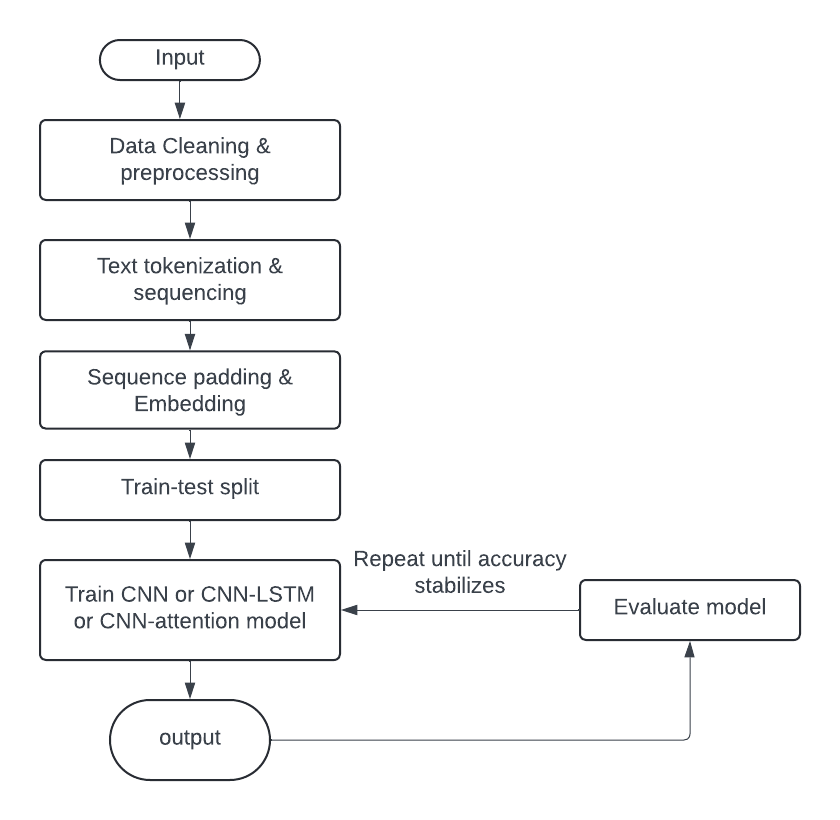
\includegraphics[scale=1.2]{model workflow.png}
    \caption{CNN model workflow}
    \label{fig:cnn workflow}
\end{figure}

\clearpage
\subsection{Dataset Description}

Input Data for this model is taken from Kaggle \cite{fake-news-dataset}, an online repository known for its diverse collection of datasets and \ac{ml} competitions. The dataset consists of 20,761 entries, with 10,387 labeled as true news and the remaining 10,374 as fake news. In this research, the text field and label field of the data are used for training the model. The label has 1 for fake news and 0 for true news.

\begin{figure}[h]
    \centering
    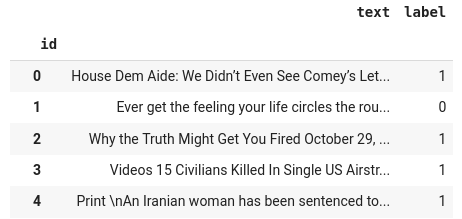
\includegraphics[scale=0.8]{dataset.png}
    \caption{Dataset structure}
    \label{fig:Dataset structure}
\end{figure}

\subsection{Data Cleaning and Preprocessing}

Data cleaning and preprocessing are done to reduce noise or irrelevant information like stopwords. It helps to standardize text by converting it to lowercase, which improves the performance of the model. The input data is passed to a function that converts text to lowercase, removes stopwords, and lemmatizes each word. Lemmatization is the process of reducing words to their base or root form, which helps in standardizing words for tasks like text analysis and \ac{nlp}.

\subsection{Tokenization and Sequencing}

To transform the text in each entry before feeding it to the CNN model, the first step is to tokenize words. Tokenization is the process of breaking down text into smaller units called tokens. These tokens can be words, subwords, or characters. The goal of tokenization is to convert raw text into a format that can be numerically processed by a neural network. Once tokenized, the tokens need to be converted into sequences of numerical values that the CNN can process.

\subsection{Padding and Embedding}

Padding is done to ensure all sequences have the same length. This is often done by padding shorter sequences with zeros or truncating longer sequences. Embedding in the context of \ac{nlp} refers to the representation of words (or tokens) as dense vectors of real numbers. These vectors capture semantic meanings and relationships between words, enabling the use of words in machine learning models. Embeddings transform words into a numerical form that preserves syntactic and semantic properties, making them suitable for neural networks and other machine learning algorithms. A pretrained \ac{glove} embedding is used. It is an unsupervised learning algorithm for obtaining vector representations for words. Unlike other word embeddings that are based solely on local context, \ac{glove} uses global statistical information from a corpus to produce dense word vectors.

\subsection{Train-Test split}

The dataset is divided into training and testing subsets. The training subset is used to train the model while the testing subset is used to evaluate the trained model using metrics like accuracy score, precision, recall, etc. 70 percent of the dataset is used for training while 30 percent is used for testing. The number of epochs is adjusted during training to assess whether the model is overfitting or underfitting.

\subsection{CNN and It's Variants}
    
    For binary classification problems such as distinguishing between Fake and True news, the mechanisms through which baseline \ac{cnn}, CNN-LSTM, and CNN-Attention models process and classify news text data are elaborated upon here. The focus is on their capability to classify text sequences as either fake or true.

    \subsubsection{\ac{cnn} model}
    \ac{cnn}s are effective at recognizing local patterns in text, such as specific phrases or word combinations, which can be indicative of fake news. It can learn discriminative features from text and can analyze the sentiment of text by detecting overly sensational or biased language often found in fake news. \\
    
    The \ac{cnn} model uses two convolution layers each followed by a dropout and max pooling layer. Dropout is used to avoid overfitting. \ac{cnn} captures the spatial pattern on text sequences which are then passed to fully connected layers to perform classification as shown in figure \ref{fig:cnn_model_architecture}. 

    \begin{figure}[h]
        \centering
        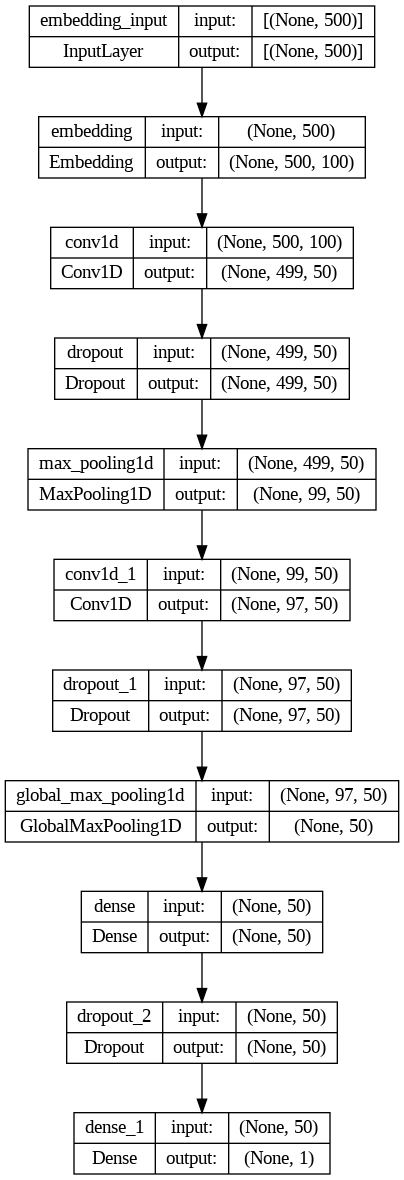
\includegraphics[scale=0.5]{CNN model arch.png}
        \caption{\ac{cnn} model architecture}
        \label{fig:cnn_model_architecture}
    \end{figure}

    \clearpage
    
    \subsubsection{CNN-LSTM model}
    It is a hybrid model that uses \ac{cnn} and \ac{lstm} layers. The pattern detected by \ac{cnn} is passed to \ac{rnn}/\ac{lstm} layer that learns the long-term dependencies of input text. \\

    \ac{lstm}s are designed to capture long-range dependencies in sequences, making them well-suited for understanding context and nuances in news articles. It helps to model the relationship between words and sentences over the entire article making them suitable to use for fake news classification.
    
    \begin{figure}[h]
        \centering
        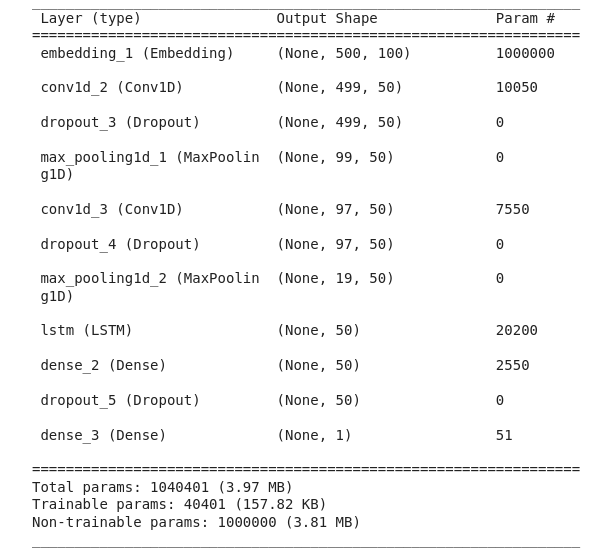
\includegraphics[scale=0.7]{CNN-LSTM-arch.png}
        \caption{CNN-LSTM model architecture}
        \label{fig:cnn-lstm-model-arch}
    \end{figure}

    \clearpage
    \subsubsection{CNN-Attention model}
    It is also a hybrid model which computes attention scores for the data generated by the CNN layer. This hybrid approach leverages the local feature extraction capabilities of CNNs and the context-awareness of attention mechanisms, making it highly effective for tasks like fake news detection.\\

    The attention mechanism calculates attention weights that signify the importance of each word (or feature) in the context of the entire article. It provides contextual information to each feature or word, which is crucial for classifying news as fake or true. The context vector is the weighted sum of the input vectors, with weights determined by the attention mechanism. The attention mechanism itself involves computing intermediate scores using a learned weight matrix W and bias vector b, applying the tanh activation function, and normalizing these scores with the softmax function to obtain the attention weights.

    \[
        \text{context} = \sum_i (\text{softmax}(\tanh(W \cdot x_i + b)) \cdot x_i)
    \]

    \begin{figure}[h]
        \centering
        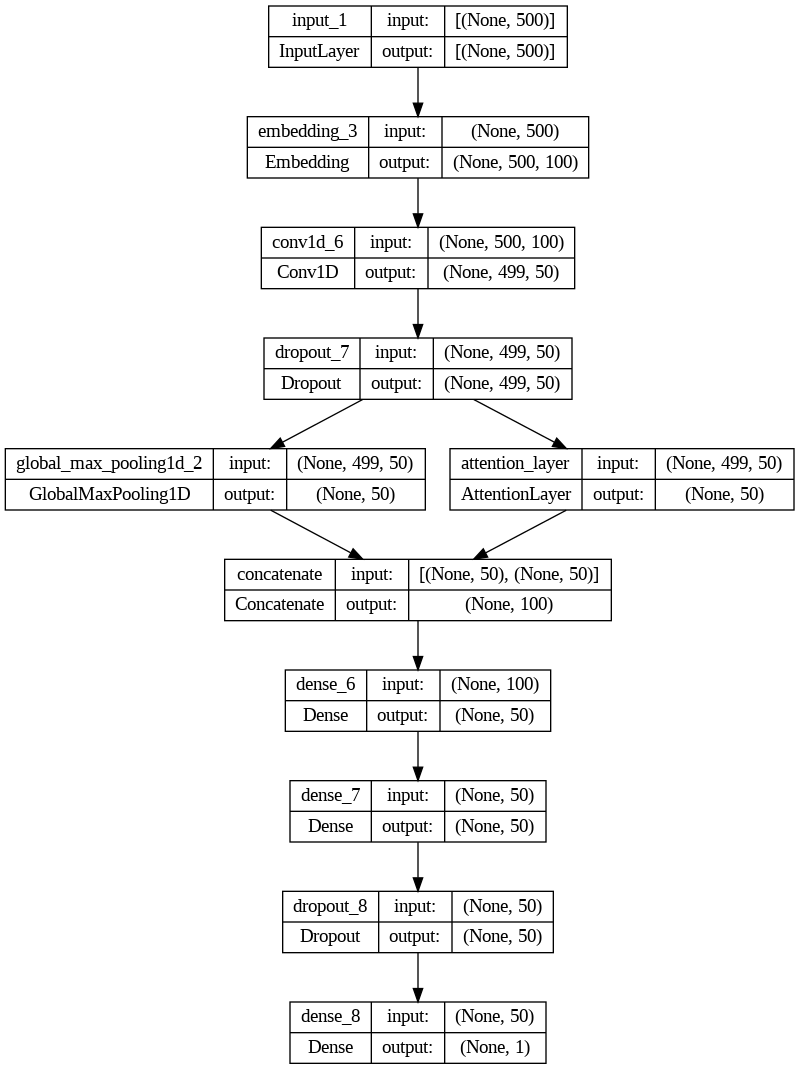
\includegraphics[scale=0.5]{CNN-Attention-arch.png}
        \caption{CNN-Attention model architecture}
        \label{fig:cnn-attention-model-arch}
    \end{figure}

\clearpage
\subsection{Evaluation}

To determine the consistency and accuracy of a classification model, typical assessment metrics are determined according to,

\begin{description}
    \item[Accuracy:] Accuracy is the ratio of correctly predicted instances to the total instances. It gives an overall measure of how often the model is correct.
    $$\text{Accuracy} = \frac{\text{True Positives} + \text{True Negatives}}{\text{Total Number of Instances}}$$

    \item[Precision:] Precision (also called Positive Predictive Value) is the ratio of correctly predicted positive observations to total predicted positives. It tells you how many of the instances predicted as positive are positive.
    $$ \text{Precision} = \frac{\text{True Positives}}{\text{True Positives} + \text{False Positives}} $$
    
    \item[Recall:]  Recall (also called Sensitivity or True Positive Rate) is the ratio of correctly predicted positive observations to all observations in the actual class. It tells you how many of the actual positive instances were captured by the model.
    $$ \text{Recall} = \frac{\text{True Positives}}{\text{True Positives} + \text{False Negatives}} $$

    \item[F1 score:] The harmonic mean of recall and precision is the F1 Score. As a result, this score takes both false positives and false negatives into account. F1 score is more useful than accuracy when the class distribution is unbalanced.
    $$ \text{F1 Score} = 2 \times \frac{\text{Precision} \times \text{Recall}}{\text{Precision} + \text{Recall}} $$
\end{description}
\clearpage

\section{Implementation}

\subsection{Implementation Tools}
Python is used as the programming language to code the program. Google Colab is used as an \ac{ide}. Similarly, different libraries are also used, such as:

\begin{description}
    \item[Tensorflow:] TensorFlow is used to build and train the CNN-based Fake News classifier.
    \item[Keras:] Keras is used to simplify the process of building and training the CNN models.
    \item[NLTK:] \ac{nltk} is a powerful library in Python for working with human language data.  It provides easy-to-use interfaces and text-processing libraries for classification, tokenization, stemming, tagging, parsing, and more.
    \item[NumPy:] NumPy is used to store and manipulate training and testing data.
    \item[Pandas:] Pandas is used to load and clean training and testing data.
    \item[Matplotlib:] Matplotlib is used to visualize the results of the Fake News classifier.
\end{description}

\subsection{Implementation Details}

\subsubsection{Data Cleaning and Preprocessing} The train and test data are passed through a function that removes stopwords, and lowercase, and then lemmatizes each word for effective learning of the model. The \ac{nltk} library is used to perform data cleaning and preprocessing.

\begin{figure}[h]
    \centering
    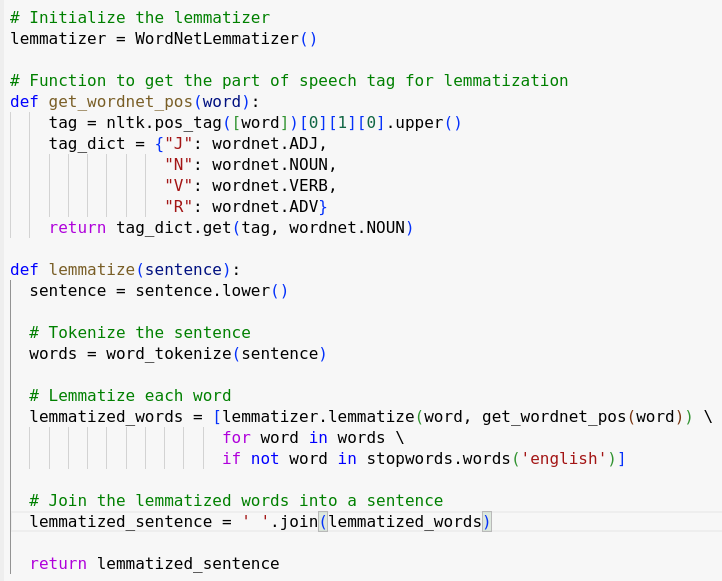
\includegraphics[scale=0.6]{Lemmatization.png}
    \caption{Python code for data cleaning and lemmatization}
    \label{fig:lemmatization}
\end{figure}

\subsubsection{Text Sequencing and Padding} The text data were transformed into sequences of words using a tokenizer, and each sequence was padded with zeros to have a fixed length of 500 words. This step ensured that all sequences had consistent dimensions for efficient processing. The sequence length of 500 words is chosen based on the experiment on the model's performance.

\begin{figure}[h]
    \centering
    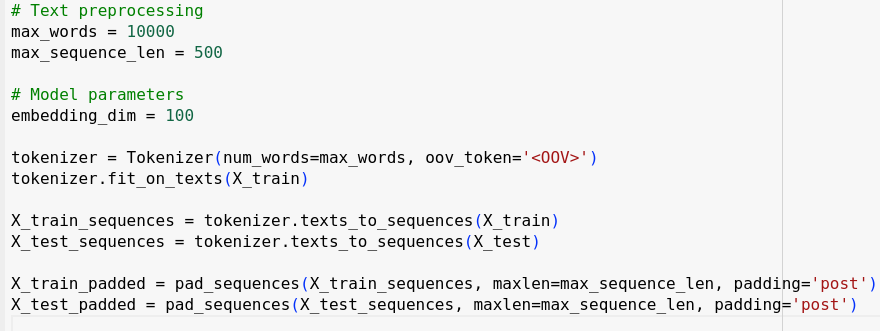
\includegraphics[scale=0.5]{sequencing_and_padding.png}
    \caption{Python code for sequencing and padding text}
    \label{fig:sequencing_and_padding}
\end{figure}

\subsubsection{Embedding} The text sequences are converted to dense 100-dimensional vectors of real numbers using \ac{glove} embedding as shown in figure \ref{fig:embedding_with_glove}. The embeddings are trained on very large text corpora which ensures embeddings generalize well to new unseen text. The pre-trained weights also help the model to train faster without compromising performance.

\begin{figure}[h]
    \centering
    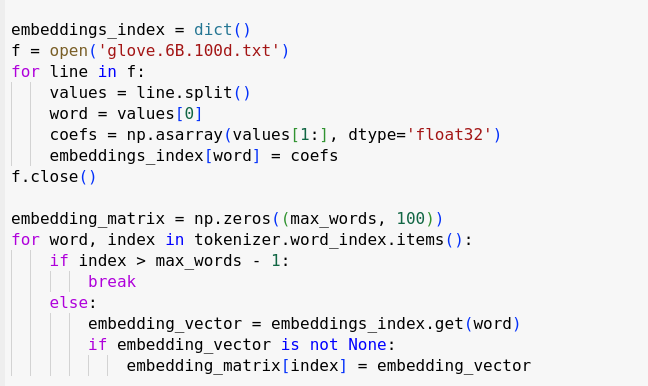
\includegraphics[scale=0.5]{embedding.png}
    \caption{Python code for generating embedding vector with GloVe}
    \label{fig:embedding_with_glove}
\end{figure}

\clearpage
\subsubsection{CNN Architecture}
\subsubsection{Baseline CNN}
The CNN model consists of an Embedding layer, and two convolutional layers followed by a pooling layer. The sequence of words is initially transformed into 100-dimensional vectors through an embedding layer, enhancing the model’s ability to process text input effectively. Dropout is used to combat overfitting in training data, finally, the model is passed to a dense layer. The convolution layer applies the filter and the Pooling layer down-samples feature maps retaining the most crucial features only. The model concludes with a softmax-activated dense layer, enabling binary classification.

\begin{figure}[ht]
    \centering
    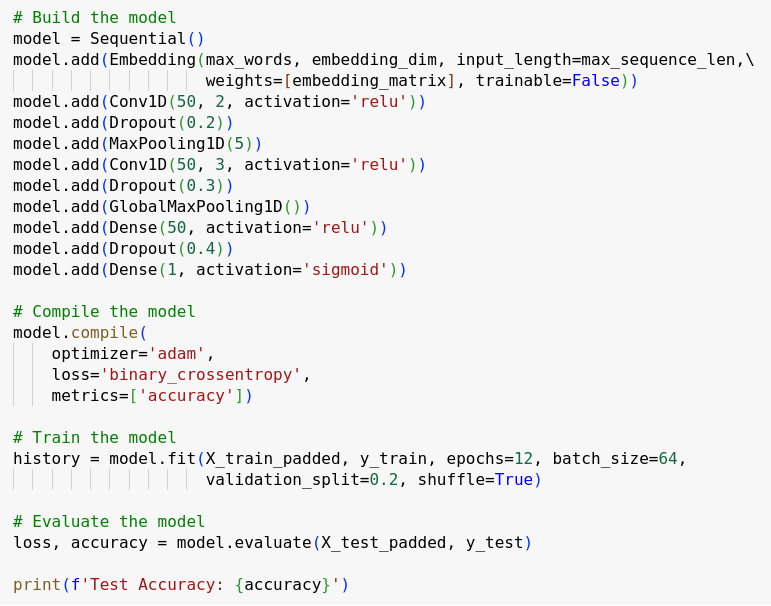
\includegraphics[scale=0.5]{cnn-implementation.png}
    \caption{CNN implementation}
    \label{fig:cnn_implementation}
\end{figure}

\clearpage

\subsubsection{CNN-LSTM}
The CNN-LSTM model uses CNN layers followed by LSTM layers. The CNN layer is similar to classic CNN architecture, LSTM layers consist of 50 units. The LSTM uses the tanh activation function and sigmoid for recurrent activation.

\begin{figure}[h]
    \centering
    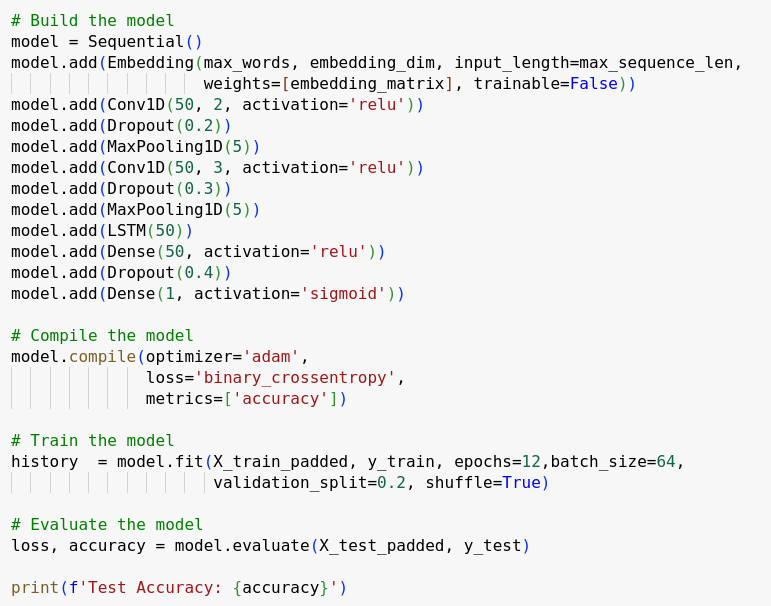
\includegraphics[scale=0.5]{cnn-lstm-implementation.png}
    \caption{CNN-LSTM implementation}
    \label{fig:cnn-lstm-implementation}
\end{figure}

\subsubsection{CNN-Attention}
The CNN-Attention model uses a CNN layer followed by an Attention layer. The Attention layer uses the output from the preceding CNN layer to compute attention weights and produce a context vector. The code to calculate attention weights is shown in figure \ref{fig:attention-implementation}.

\begin{figure}[h]
    \centering
    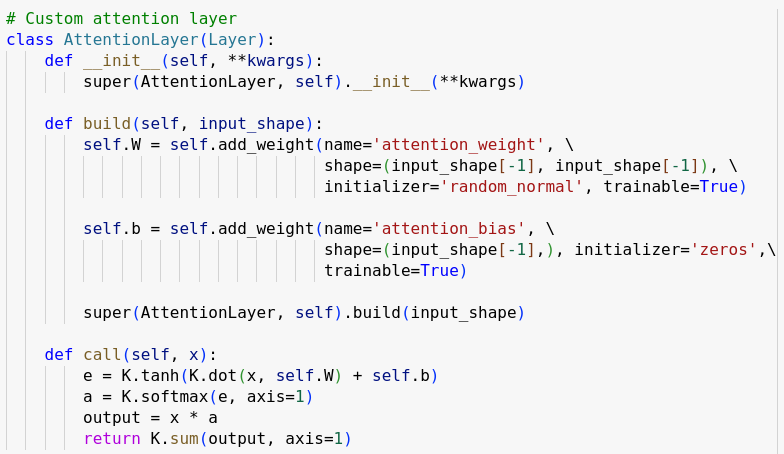
\includegraphics[scale=0.5]{attention_implementation.png}
    \caption{Attention implementation}
    \label{fig:attention-implementation}
\end{figure}

\begin{figure}[h]
    \centering
    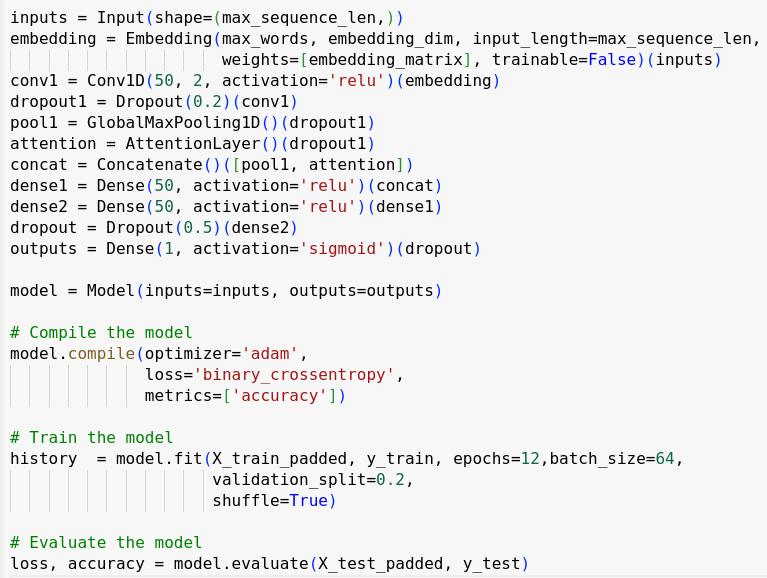
\includegraphics[scale=0.5]{cnn-attention-implementation.png}
    \caption{CNN-Attention implementation}
    \label{fig:cnn-attention-implementation}
\end{figure}

\clearpage
\subsubsection{Model Optimization and Training} 
For model optimization, the Adam optimizer and binary cross-entropy loss function were utilized. The evaluation metrics included accuracy, precision, and recall. The models were trained for 12 epochs.

\subsubsection{Model Evaluation} 
The models' performance is assessed using a test dataset by generating categorical predictions through the \lq predict\rq\  method. These predictions are compared to actual labels to form a confusion matrix, from which accuracy, precision, and recall are calculated to evaluate the models' effectiveness in classifying true or fake news.

\begin{figure}[h]
    \centering
    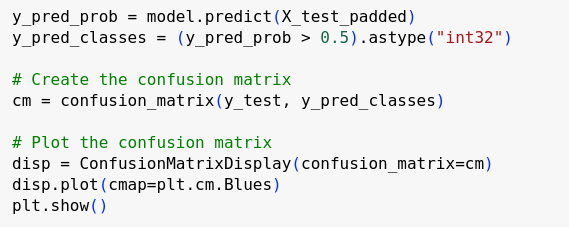
\includegraphics[scale=0.65]{confusiong matrix code.png}
    \caption{Code for confusion matrix}    
\end{figure}

\section{Findings and Result}

\subsection{Confusion Matrix}
The confusion matrix displays the performance evaluation of a classification model on a test dataset. It consists of actual classes and predicted classes.

\subsubsection{Confusion matrix of Baseline CNN}

\begin{description}
    \item[True Positives (TP):] There are 2951 true positives, correctly predicting ‘Fake’.
    \item[False Negatives (FN):] There are 161 false negatives, incorrectly predicting ‘Fake’.
    \item[False Positives (FP):] There are 95 false positives, incorrectly predicting 'True'.
    \item[True Negatives (TN): ] There are 2999 true negatives, correctly predicting ‘True’.
\end{description}

\begin{figure}[h]
    \centering
    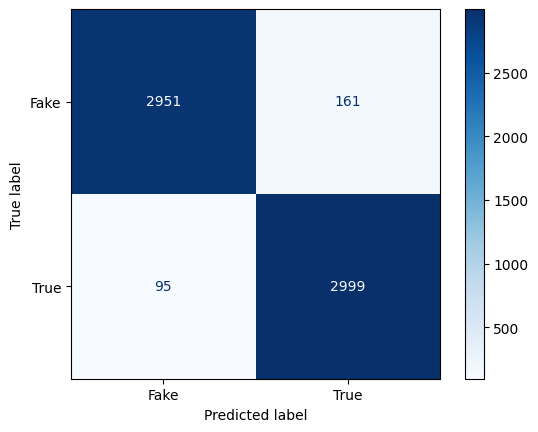
\includegraphics[scale=0.65]{cm_baseline_cnn.png}
    \caption{Confusion matrix of baseline CNN}    
\end{figure}

% \clearpage
\subsubsection{Confusion matrix of CNN-LSTM}

\begin{description}
    \item[True Positives (TP):] There are 3028 true positives, correctly predicting ‘Fake’.
    \item[False Negatives (FN):] There are 84 false negatives, incorrectly predicting ‘Fake’.
    \item[False Positives (FP):] There are 143 false positives, incorrectly predicting 'True'.
    \item[True Negatives (TN): ] There are 2951 true negatives, correctly predicting ‘True’.
\end{description}

\begin{figure}[h]
    \centering
    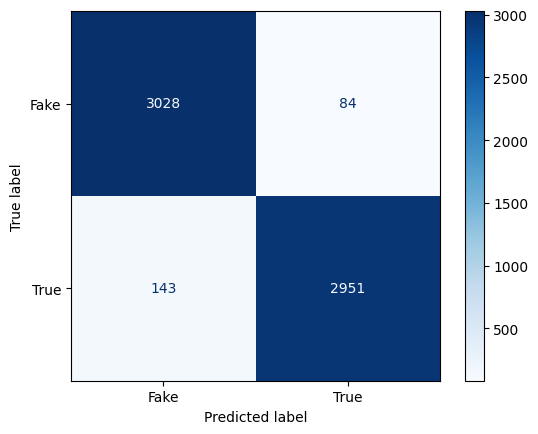
\includegraphics[scale=0.65]{cm_cnn-lstm.png}
    \caption{Confusion matrix of CNN-LSTM}
    \label{fig:cm_cnn-lstm}
\end{figure}
\clearpage
\subsubsection{Confusion matrix of CNN-Attention}

\begin{description}
    \item[True Positives (TP):] There are 3039 true positives, correctly predicting ‘Fake’.
    \item[False Negatives (FN):] There are 73 false negatives, incorrectly predicting ‘Fake’.
    \item[False Positives (FP):] There are 104 false positives, incorrectly predicting 'True'.
    \item[True Negatives (TN): ] There are 2990 true negatives, correctly predicting ‘True’.
\end{description}

\begin{figure}[h]
    \centering
    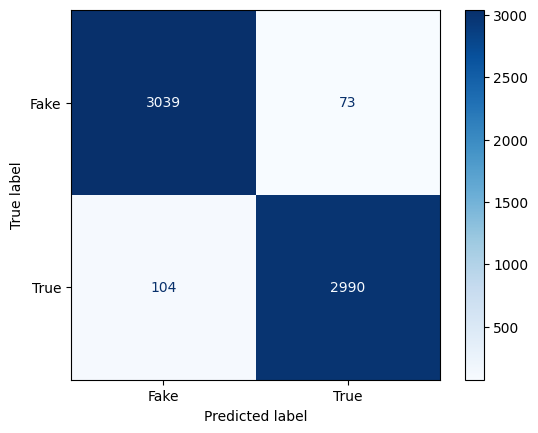
\includegraphics[scale=0.65]{cm_cnn-attention.png}
    \caption{Confusion matrix of CNN-Attention}
    \label{fig:cm_cnn-attention}
\end{figure}


% \clearpage
\subsection{Accuracy Parameters} 
The accuracy parameters using \ac{cnn} variants are evaluated on the test dataset. The observations are listed below:

\begin{table}[h]
    \caption{Accuracy parameters of CNN variants}
    \centering
    \begin{tabular}{|c|c|c|c|}
    \hline
      \textbf{Model} & \textbf{CNN} & \textbf{CNN-LSTM} & \textbf{CNN-Attention} \\
      \hline
        \textbf{Accuracy} &95.87\%  &96.34\% & 97.14\%\\
        \hline
        \textbf{Precision} & 96\%& 96\%&97\% \\
        \hline
        \textbf{Recall} & 96\%&96\% &97\% \\
       \hline
       \textbf{F1 score} & 96\%&96\% &97\% \\
       \hline
    \end{tabular} 
   
    \label{tab:accuracy_params_of_cnn_variants}
\end{table}

Comparing \ac{cnn} and its variants, there is stable precision and recall while precision, recall, and accuracy slightly increase for the CNN-Attention variant. Based on accuracy parameters CNN-Attention has performed better.
\clearpage

\subsection{Overfitting and Generalization} 
The training and validation loss and accuracy plots demonstrated a smooth convergence throughout the training process, indicating that the model effectively learned from the data without signs of overfitting or underfitting.

\begin{figure}[h]
    \centering
    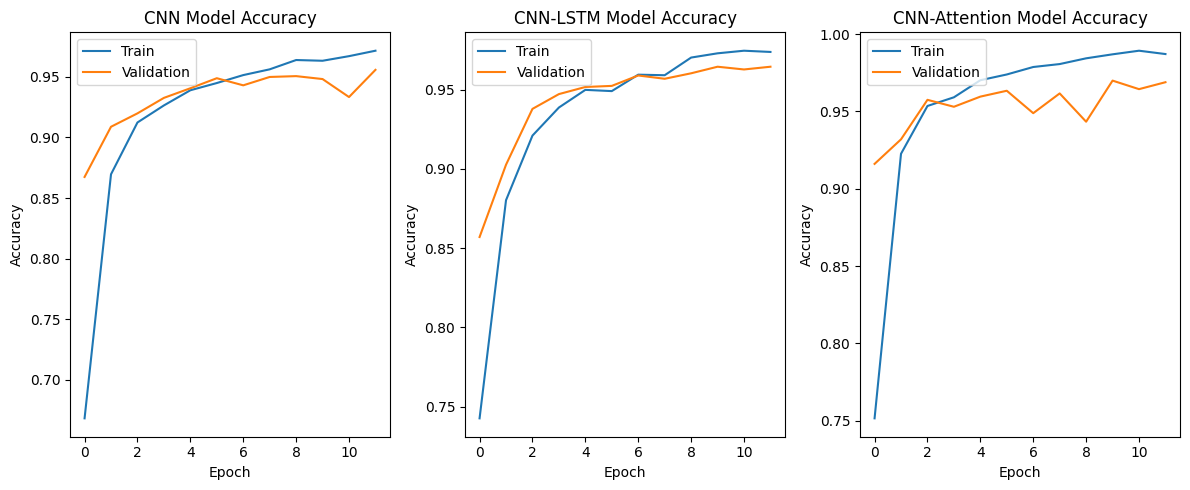
\includegraphics[scale=0.52]{accuracy images.png}
    \caption{Training and validation accuracy over epochs for CNN, CNN-LSTM, and CNN-Attention}  
\end{figure}

\begin{figure}[h]
    \centering
    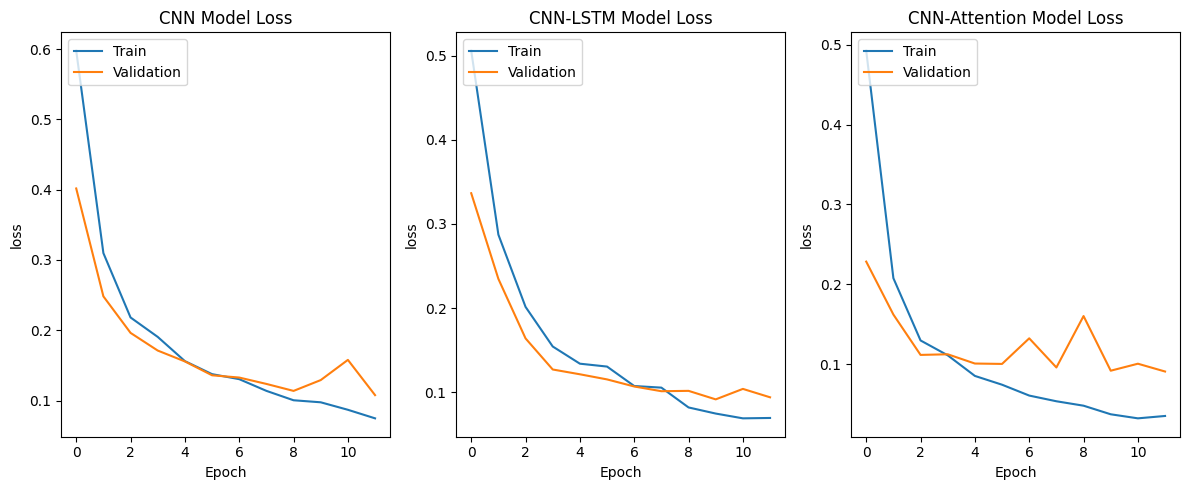
\includegraphics[scale=0.52]{loss images.png}
    \caption{Training and validation loss over epochs for CNN, CNN-LSTM, and CNN-Attention}   
\end{figure}
\clearpage
\subsection{Result Analysis}
The accuracy, precision, and recall observed on various \ac{cnn} models suggest that the local patterns detected by baseline \ac{cnn} like specific words or phrase combinations are enough for fake news classification. The long-range dependencies by the LSTM layer did not increase accuracy by a significant amount compared to the CNN-Attention model, which suggests long-range dependencies are not critical or enough for the task on the current dataset. Better performance of CNN-Attention, +0.8\% accuracy than CNN-LSTM and +1.3\% accuracy than baseline CNN suggest, focusing on informative parts of the text by dynamically weighing using attention mechanism can enhance model performance. It highlights the fact that adding contextual information to words using an attention mechanism is indeed useful. \\

The training and validation accuracy and loss over epoch are similar on all models suggesting, that all models are converging to a similar level of performance. Models are learning effectively from the data and are not significantly overfitting or underfitting. The models converges at 12\textsuperscript{th} epoch.

